\subsection{Impact of Individual Techniques}
\label{exp:indiv}

%\begin{figure}
%	\centering
%	\subfigure[RTE]{
%		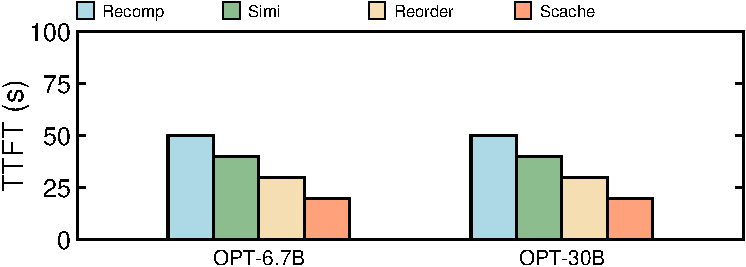
\includegraphics[width=1.5in, height=1in]{indiv_ds1.pdf}
%		\label{fig:indiv_ds1}
%	}
%	\hspace{0.06in}
%	\subfigure[COPA]{
%		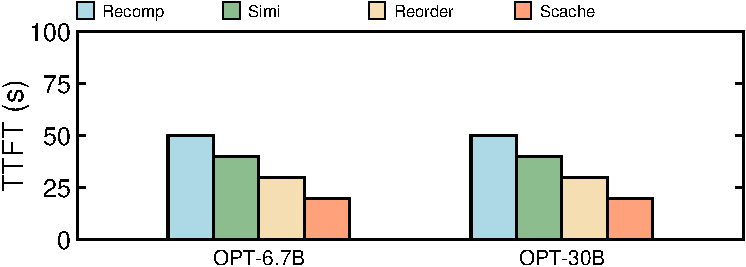
\includegraphics[width=1.5in, height=1in]{indiv_ds2.pdf}
%		\label{fig:indiv_ds2}
%	}
%	\vspace{-0.2in}
%	\caption{
%		The performance impact of each optimizatio.}
%	\label{fig:indiv}
%\end{figure}

%Figure~\ref{fig:indiv} illustrates the impact of each optimization in \pname{}.
%We use the current SOTA system \textit{AS+H2O+LFU} as the baseline and normalize
%its TTFT to one. \textit{+ITF} represents the version which enhances baseline
%with \techa{}, which only loads important KVs; \textit{+RO} builds upon
%\textit{+ITF} by enabling the \techba{} technique; \textit{All} refers to the
%version that further incorporates the \techbb{} strategy on top of
%\textit{+RO}. 
\fvc{
Figure~\ref{fig:indiv} shows the impact of each optimization. Using the current SOTA system \textit{AS+H2O+LFU} as the baseline (TTFT normalized to one), \textit{+ITF} adds \techa{} for loading important KVs, \textit{+RO} enables \techba{} on \textit{+ITF}, and \textit{All} incorporates \techbb{} on \textit{+RO}.
}
%Due to space limitations, we only present the results of
%two models and two datasets.
%From the figure, we have two findings. First, we observe that each optimization further reduces TTFT, with \textit{All}
%achieving the shortest TTFT. This demonstrates the effectiveness of each
%individual technique in \pname{}. 
%Second, the contributions of different techniques vary across models and datasets. For instance, in OPT-30B on the RTE dataset, the respective contributions of the three techniques are 60\%, 30\%, and 10\%. In contrast, on the COPA dataset with OPT-13B, the contributions are 36\%, 8\%, and 56\%, respectively.
\fvc{
We observe that each optimization reduces TTFT, with \textit{All} achieving the shortest TTFT, showing the effectiveness of \pname{}'s individual techniques. Besides, technique contributions vary across models and datasets. For example, in OPT-30B on RTE, the contributions of the three techniques are 60\%, 30\%, and 10\%, while on COPA with OPT-13B, they are 36\%, 8\%, and 56\%.
}


% To understand the impact of each optimization on OPT-30B,
% Figure~\ref{fig:indiv_a} shows the average ratio of KVs loaded at each layer for
% OPT-30B on
% PIQA dataset in \textit{+ITF} sytem. 
% \textit{+ITF} can dynamically decide whether to load partial or full KVs for different layers, striking a balance between model accuracy and TTFT.
% Figure~\ref{fig:indiv_b} shows that, after enabling \techba{}, the number of
% loaded chunks decreases by an average of 1.2$\times$. This is because important
% keys and values are placed in the same chunk, reducing the number of chunks that
% need to be loaded for reusing important token KVs. 
% This result indicates the effectiveness of \techba{}.
% Figure~\ref{fig:indiv_c}shows the change in GPU hit ratio after enabling the
% \techbb{} technique. It reveals that the average GPU hit ratio increases from
% 68\% to 80\% across the four datasets. This reduces PCIe data transfer, which
% explains why \textit{All} achieves the lowest TTFT.

Figure~\ref{fig:indiv_a} shows the average KV loading ratio per layer for OPT-30B on the PIQA dataset using the \textit{+ITF} system, which dynamically adjusts KV loading to optimize the trade-off between accuracy and TTFT.
Figure~\ref{fig:indiv_b} indicates that enabling \techba{} results in an average 1.2$\times$ reduction in loaded chunks, as it consolidates important keys and values into fewer chunks.
%, streamlining the loading process for important token KVs.
Figure~\ref{fig:indiv_c} shows that \techbb{} boosts the average GPU hit ratio from 68\% to 80\% across four datasets, thereby reducing PCIe data transfers.
%and contributing to the lowest TTFT in the \textit{All} configuration.


\begin{figure}
	\centering
	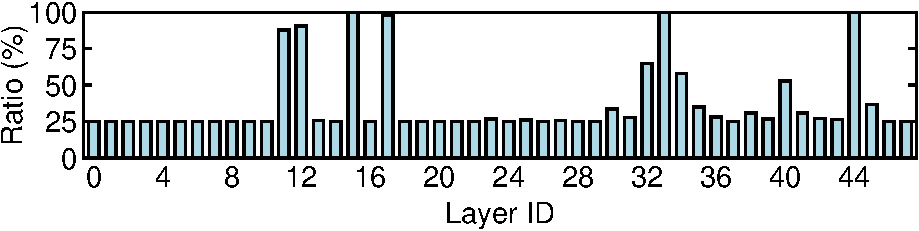
\includegraphics[width=3.3in, height=0.8in]{indiv_a_ds1.pdf}
	\vspace{-0.1in}
	\caption{The retention of KVs per model layer using \techa{}.}
	\label{fig:indiv_a}
	 \vspace{-0.1in}
\end{figure}


\begin{figure}
	\centering
	\begin{minipage}{1.6in}
		% \centering
		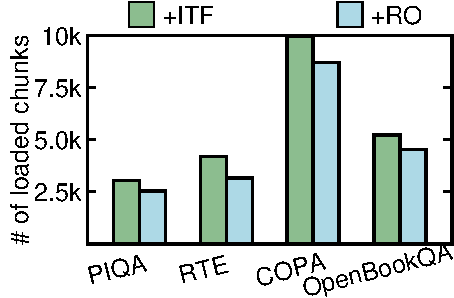
\includegraphics[width=1.6in,height=1in]{indiv_b_cknum.pdf}
		\vspace{-0.2in}
		\caption{
			The impact of \techba{} on the number of loaded chunks.
		}
		\label{fig:indiv_b}
	\end{minipage}
	\hspace{0.05in}
	\begin{minipage}{1.6in}
		\centering
		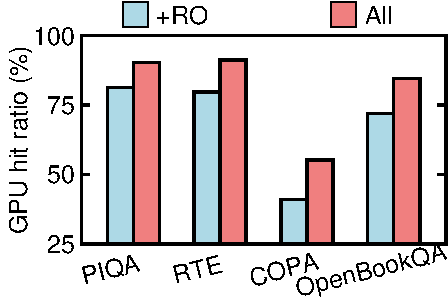
\includegraphics[width=1.6in, height=1in]{indiv_c_13b.pdf}
		\vspace{-0.2in}
		\caption{
			The impact of scored-based cache management on GPU hit ratios.
		}
		\label{fig:indiv_c}
	\end{minipage} 
	\vspace{-0.2in}
\end{figure}




%\begin{figure}
%	\centering
%	\subfigure[Number of loaded chunks]{
%		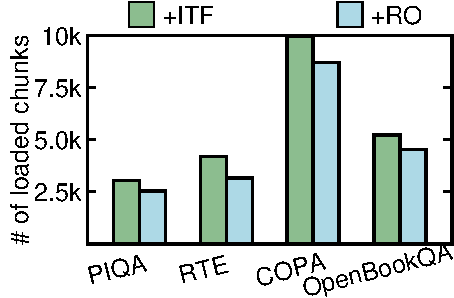
\includegraphics[width=1.5in, height=1in]{indiv_b_cknum.pdf}
%	}
%	\hspace{0.06in}
%	\subfigure[Important KV ratio]{
%		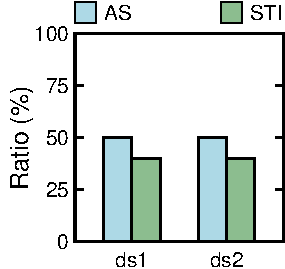
\includegraphics[width=1.5in, height=1in]{indiv_b_ckratio.pdf}
%		\label{fig:indiv_b_ratio}
%	}
%	\vspace{-0.1in}
%	\caption{
%		Comparison of the total number of loaded chunks and the average important KV ratio in each chunk before and after using \techba{}.}
%	\label{fig:indiv_b}
%\end{figure}


%\begin{figure}
%	\centering
%	\subfigure[ds1]{
%		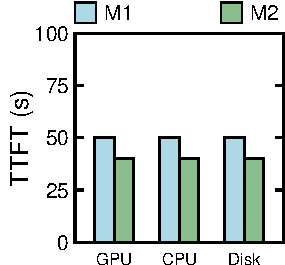
\includegraphics[width=1.5in, height=1in]{indiv_c_ds1.pdf}
%	}
%	\hspace{0.06in}
%	\subfigure[ds2]{
%		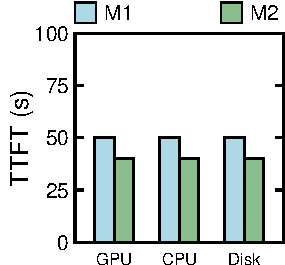
\includegraphics[width=1.5in, height=1in]{indiv_c_ds2.pdf}
%	}
%	\vspace{-0.1in}
%	\caption{
%		Comparison of the cache hit ratios.}
%	\label{fig:indiv_c}
%\end{figure}
